\beginsong{Avondlied}
\beginverse
O Heer, d'avond is neergekomen. De zonne zonk, het duister klom. De winden doorruisen de bomen. En verre sterren staan alom. Wij knielen neer om U te zingen. In't slapend woud ons avondlied. Wij danken U voor wat we ontvingen. En vragen, Heer, verlaat ons niet.
\endverse
\beginchorus
Scouts en leiders knielen wij neder. Door de stilte weerklinkt onze bee. Luistrend fluistren kruinen mee. En sterren staren teder. Geef ons, Heer, zegen en rust en vree...
\endchorus
\beginverse
Gij hebt dezen dag ons gegeven. En ons bewaard gezond en blij. Uw engel is ons bijgebleven. En heeft gewandeld aan ons zij! We deden goed met uw genaden. We leerden menig wijze raad. Eenieder heeft door woord en daden. Zijn makkers broederlijk gebaat!
\endverse
\beginverse
Al wat wij boos en zwak misdeden. Vergeef het ons, O goede Heer. Uw liefde heeft voor ons geleden. Wees ons barmhartig nog een keer... Wij willen weer U trouw beloven. Ons Woord vernieuwen, Heer, voor U. En zeker van Uw hulp van boven. Laat ons gelukkig slapen nu!
\endverse
\beginverse
Weleer toen uw apostlen sliepen, toen badt G'op enen berg alleen. Waak over ons, die U aanriepen. Drijf duivel, dood en vijand heen... Waak over ons, Gij, Licht en Leven, Gij Waarheid, en 'ge Levensbaan. En morgen wordt U weer gegeven, Elke avond, ieder zonopstaan!
\endverse
\endsong
\begin{intersong}
    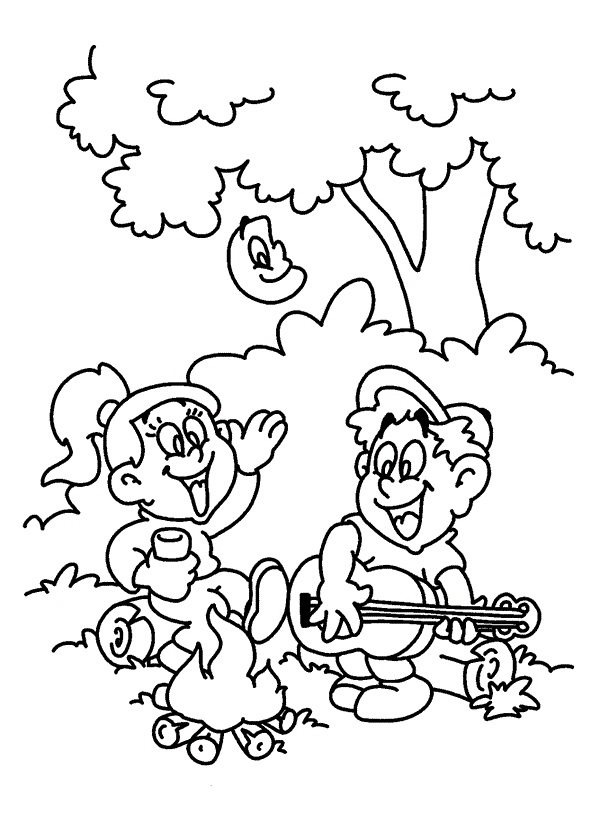
\includegraphics[width=0.4\textwidth]{img6}
\end{intersong}